\subsection{Driving the Segments}
%Open the arduino software.  Check if the ports show Arduino Uno and click the appropriate button.  
\begin{problem}
%Connect the A-D pins of the 7447 IC to the pins D2-D5 of the Arduino.
%Connect the A-D pins of the 7447 IC  in Fig. \ref{fig:7447} to the GPIO pins  0-3 of the Pi shown in Figs. \ref{fig_1_3a} and \ref{fig_1_3b}.
\end{problem}	
\renewcommand{\thefigure}{\theproblem.\arabic{figure}}
\begin{figure}[!ht]
\begin{center}
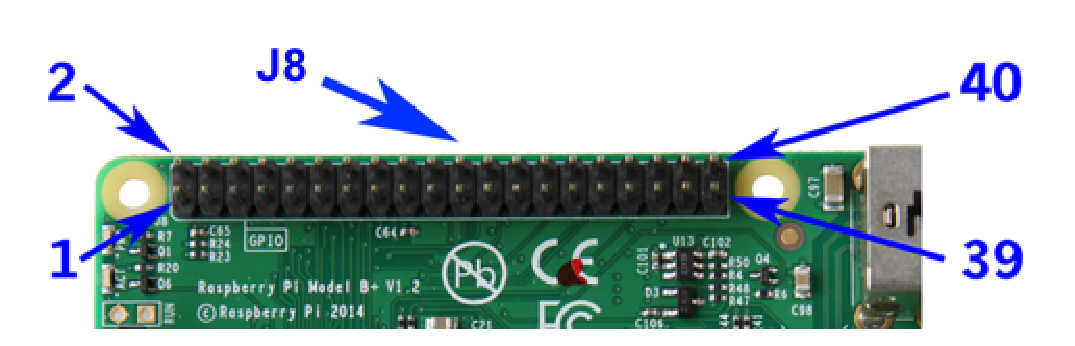
\includegraphics[width=\columnwidth]{./figs/gpio2}
\end{center}
\captionof{figure}{GPIO pin snapshot on Pi.}
\label{fig_1_3a}	
\end{figure}
%
\begin{figure}
\begin{center}
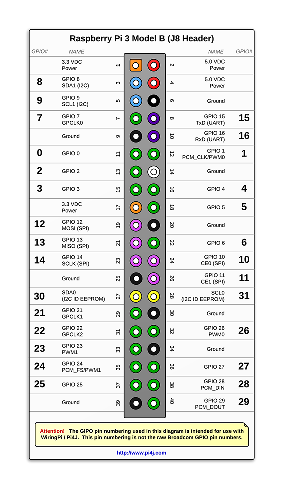
\includegraphics[width=\columnwidth]{./figs/gpio1}
\end{center}
\captionof{figure}{GPIO Wiring Pi pin configuration.}
\label{fig_1_3b}	
\end{figure}
\renewcommand{\thefigure}{\theproblem}
\begin{problem}
Connect the a-g pins of the display to the GPIO pins 0-6 of the Pi shown in \ref{fig_1_3a} and \ref{fig_1_3b}.
\end{problem}
\begin{problem}
Type the following C code and excute. What do you observe?
\end{problem}
\solution
\lstinputlisting[language=C]{./code/seven_seg_disp.c}
\begin{problem}
Now generate the numbers 0-9 by modifying the above program.
\end{problem}
\begin{problem}
Suitably modify the above program to obtain a decade counter.
\end{problem}


%\begin{problem}
%\label{prob:first_code}
%%Type the following code and execute. What do you observe?
%%\lstinputlisting[language=C]{./codes/bcd_seven.c}
%%// the setup function runs once when you press reset or power the board
int a=1,b=0,c=0,d=1,e=1,f=1,g=1;
void setup() {
    pinMode(2, OUTPUT);  
    pinMode(3, OUTPUT);
    pinMode(4, OUTPUT);
    pinMode(5, OUTPUT);
    pinMode(6, OUTPUT);
    pinMode(7, OUTPUT);
    pinMode(8, OUTPUT);            
}

// the loop function runs over and over again forever
void loop() {
  
  digitalWrite(2, a); 
  digitalWrite(3, b); 
  digitalWrite(4, c); 
  digitalWrite(5, d); 
  digitalWrite(6, e); 
  digitalWrite(7, f);     
  digitalWrite(8, g); 
}


%\end{problem}
%\begin{problem}
%Now generate the numbers 0-9 by modifying the above program.
%\end{problem}
%%
%%\newpage

%%\section{Combinational Logic}
%%
%\subsection{Counting Decoder}
	%In the  truth table in Table \ref{table:counter_decoder},  $W,X,Y,Z$ are the inputs
%and $A,B,C,D$ are the outputs. This table represents the system that increments the numbers 0-8 by 1 and resets the number 9 to 0
%%
%Note that  $D = 1$ for the inputs $0111$ and $1000$.  Using {\em boolean} logic,
%%
%\begin{equation}
%\label{bool_logic}
%D = WXYZ^{'} + W^{'}X^{'}Y^{'}Z
%\end{equation}
%%
%Note that $0111$ results in the expression $WXYZ^{'}$ and $1000$ yields $W^{'}X^{'}Y^{'}Z$. 
%%The $\&\&$ operand is used for the boolean AND (multiplication) operation, the $||$ operand is used for the OR (addition) operation and the ! operand is used for the NOT ($^{'}$) operation in Arduino code.  For example, the expression for \eqref{bool_logic} in Arudino is
%%\begin{verbatim}
%%D = (W&&X&&Y&&!Z)||(!W&&!X&&!Y&&Z);
%%\end{verbatim}

%\begin{problem}
	%\label{counter_dec}

%Write the boolean logic functions for $A,B,C$ in terms of $W,X,Y,Z$.
%\end{problem}
%%
%\input{./figs/counter_decoder}
%%
%%
%\begin{problem}
%%	\label{D_code}
%Write a program for implementing Table \ref{counter_dec}.
%%\eqref{bool_logic} in Arduino.
%\end{problem}
%%
%\solution
%%\lstinputlisting[language=C]{./codes/count_decoder.c}
%%
%%\begin{problem}
%%Modify the above program by keeping W=0,X=0,Y=0,Z=1 and A=1 and execute.  Verify that your results are consistent with Table \ref{counter_dec}.
%%\end{problem}

%\begin{problem}
%Verify if your logic is correct by observing the output on the seven segment display for different inputs.
%\end{problem}
%%
%\begin{problem}
%Connect GPIO pin 10 to the dot pin of the display and execute the following code.
%\end{problem}
%%\lstinputlisting[language=C]{./codes/blink.c}
%%
%%
%\begin{problem}
%A decade counter counts the numbers from 0-9 and then resets to 0.  Suitable modify the above programs to obtain a decade counter.
%\end{problem}

%\subsection{Display Decoder}
%%
%\begin{problem}
%Now write the truth table for the seven segment display decoder (IC 7447).  The inputs will be $A,B,C,D$ and the outputs will be $a,b,c,d,e,f,g$.
%\end{problem}
%%
%\begin{problem}
%\label{seven_seg_disp_logic}
%Obtain the logic functions for outputs $a,b,c,d,e,f,g$ in terms of the inputs $A,B,C,D$.
%\end{problem}
%\begin{problem}
%Disconnect the Pi from IC 7447 and connect the pins GPIO 0-6 in the Pi directly to the seven segment display.
%\end{problem}
%\begin{problem}
%Write a new program to implement the logic in Problem \ref{seven_seg_disp_logic} and observe the output in the display.  You have designed the logic for IC 7447!
%\end{problem}
%\begin{problem}
%Now include your counting decoder program in the  display decoder program
%and see if the display shows the consecutive number.
%\end{problem}
%A decade counter counts the numbers from 0-9 and then resets to 0.
%\begin{problem}
%Suitably modify the above program to obtain a decade counter.
%\end{problem}




%\begin{problem}
%Generate the boolean functions for the segments $a-f$ using the table in Problem \ref{bcd_ss}.  For example, the function for $a$ is obtained from the table as
%\begin{equation}
%a=\bar{D}\bar{C}\bar{B}A+\bar{D}C\bar{B}\bar{A}
%\label{boolean}
%\end{equation}
%\end{problem}
%%
%\begin{problem}
	%\label{counter_dec}
%Write functions for $A,B,C,D$ in Arduino using the following table and verify using the Arduino driven display.
		%\input{counter_decoder}
%\end{problem}
%\begin{problem}
	%Write a module for decimal to binary conversion
	%according to the example given below
	%\input{conversion}
	%%
	%$N \% 2$ gives the remainder and $N/2$ gives the quotient
%	and use it in the above code so that decimal values are given as input in the program and observed as output in the display. Note that the following code
%	\begin{verbatim}
%	a % b
%	\end{verbatim}
%	can be used to obtain the remainder when a is divided by b and
%	\begin{verbatim}
%	a/b
%	\end{verbatim}
%	gives the quotient.
%\end{problem}
